\documentclass[11pt]{beamer}

% Theme selection
\usetheme{Madrid}
\usecolortheme{default}

% Configure the template
\beamertemplatenavigationsymbolsempty
\setbeamertemplate{footline}[page number]
\setbeamertemplate{enumerate items}[default]
\setbeamertemplate{caption}[numbered]
\setbeamerfont{caption}{size=\small}

% Packages
\usepackage[utf8]{inputenc}

% Links
\usepackage{hyperref}
\setlength\itemsep{2em}
\hypersetup{
  colorlinks=true,
    linkcolor=blue,
    filecolor=magenta,
    urlcolor=blue!80,
  }
\urlstyle{same}

% Images
\usepackage{graphicx}
\usepackage{caption}
\usepackage{subcaption}

%\usepackage{enumitem} % fails with beamer
\usepackage[outputdir=aux]{minted}
\usepackage[svgnames]{xcolor}

% For \titlepage
\title{Convolutional Networks and Autoencoders}
\author{Santiago Miranda}
\institute{PhD Application}
\date{March 12, 2026}

% Shortcuts
\NewDocumentCommand{\frameworksize}{}{1em}
\NewDocumentCommand{\github}{}{
\includegraphics[width=0.8em]{./pdf/github.pdf}}
\NewDocumentCommand{\npm}{}{
\includegraphics[width=0.8em]{./pdf/npm.pdf}}
\NewDocumentCommand{\tf}{}{
\includegraphics[width=\frameworksize]{./pdf/tensorflow.pdf}}
\NewDocumentCommand{\pytorch}{}{
\includegraphics[width=\frameworksize]{./pdf/pytorch.pdf}}

% Downloads
\NewDocumentCommand{\downloadsize}{}{5.5em}
\NewDocumentCommand{\hs}{}{\hspace{0em}}
\NewDocumentCommand{\wdf}{}{\hs
\includegraphics[width=\downloadsize]{./pdf/wdf-parser_downloads.pdf}}
\NewDocumentCommand{\spc}{}{\hs
\includegraphics[width=\downloadsize]{./pdf/spc-parser_downloads.pdf}}
\NewDocumentCommand{\iobuffer}{}{\hs
\includegraphics[width=\downloadsize]{./pdf/iobuffer_downloads.pdf}}
\NewDocumentCommand{\fcnnls}{}{\hs
\includegraphics[width=\downloadsize]{./pdf/fcnnls_downloads.pdf}}
\NewDocumentCommand{\regression}{}{\hs
\includegraphics[width=\downloadsize]{./pdf/regression-simple-linear_downloads.pdf}}
\NewDocumentCommand{\regressionp}{}{\hs
\includegraphics[width=\downloadsize]{./pdf/regression-polynomial.pdf}}

\begin{document}
\frame{\titlepage}

% begin-frame-title
% What I will talk about.
\begin{frame}{Previous Work}
  \begin{itemize}[<+->]
  \item Neural Networks,
    \begin{enumerate}
    \setlength\itemsep{0.3em}
    \item[a)] Inverse design with autoencoders,
    \item[b)] Object detection with convolutional networks,
    \end{enumerate}
  \setlength\itemsep{1em}
  \item Binary parsers for chemical data,
  \item \color<6->{gray} Mathematical optimisation.
  \end{itemize}
\end{frame}


\begin{frame}{Generative AI}
  Outline and results:\footnote{Done at the University of Glasgow.}
\vspace{1em}

\textit{Completed} (first 2--3 months):

\begin{description}
   \item[Survey] deep learning models $\rightarrow$ selected VAE (Fig. \ref{fig:VAE}),
   \item[Implement] simplified model (Keras 3),
   \item[Deploy] quantise model ONNX model in browser,
   \item[Package] document, test, notebooks.
\end{description}
\pause

\vspace{1em}

\textit{Planned}:
\begin{description}
  \item[Optimise] UV HOMO-LUMO gap,
  \item[Select] candidate for robotic synthesis.
\end{description}
\end{frame}

\begin{frame}{Generative AI - Inspiration}
\begin{figure}
    \begin{subfigure}[h]{0.4\textwidth}
    \flushleft
      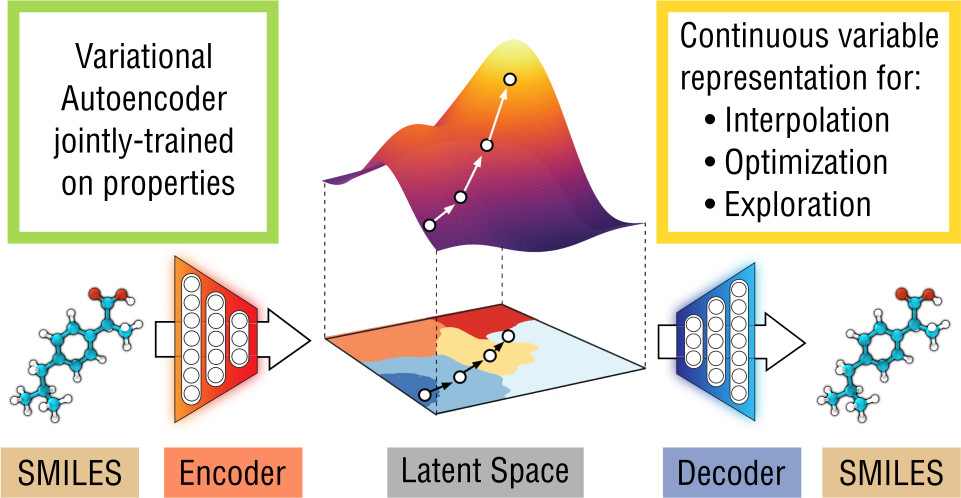
\includegraphics[width=\textwidth]{./jpeg/CVAE.jpeg}
      \caption{VAE: Aspuru-Guzik et. al.\label{fig:VAE}}
    \end{subfigure}
    \hspace{1em}
    \pause
    \begin{subfigure}[h]{0.5\textwidth}
      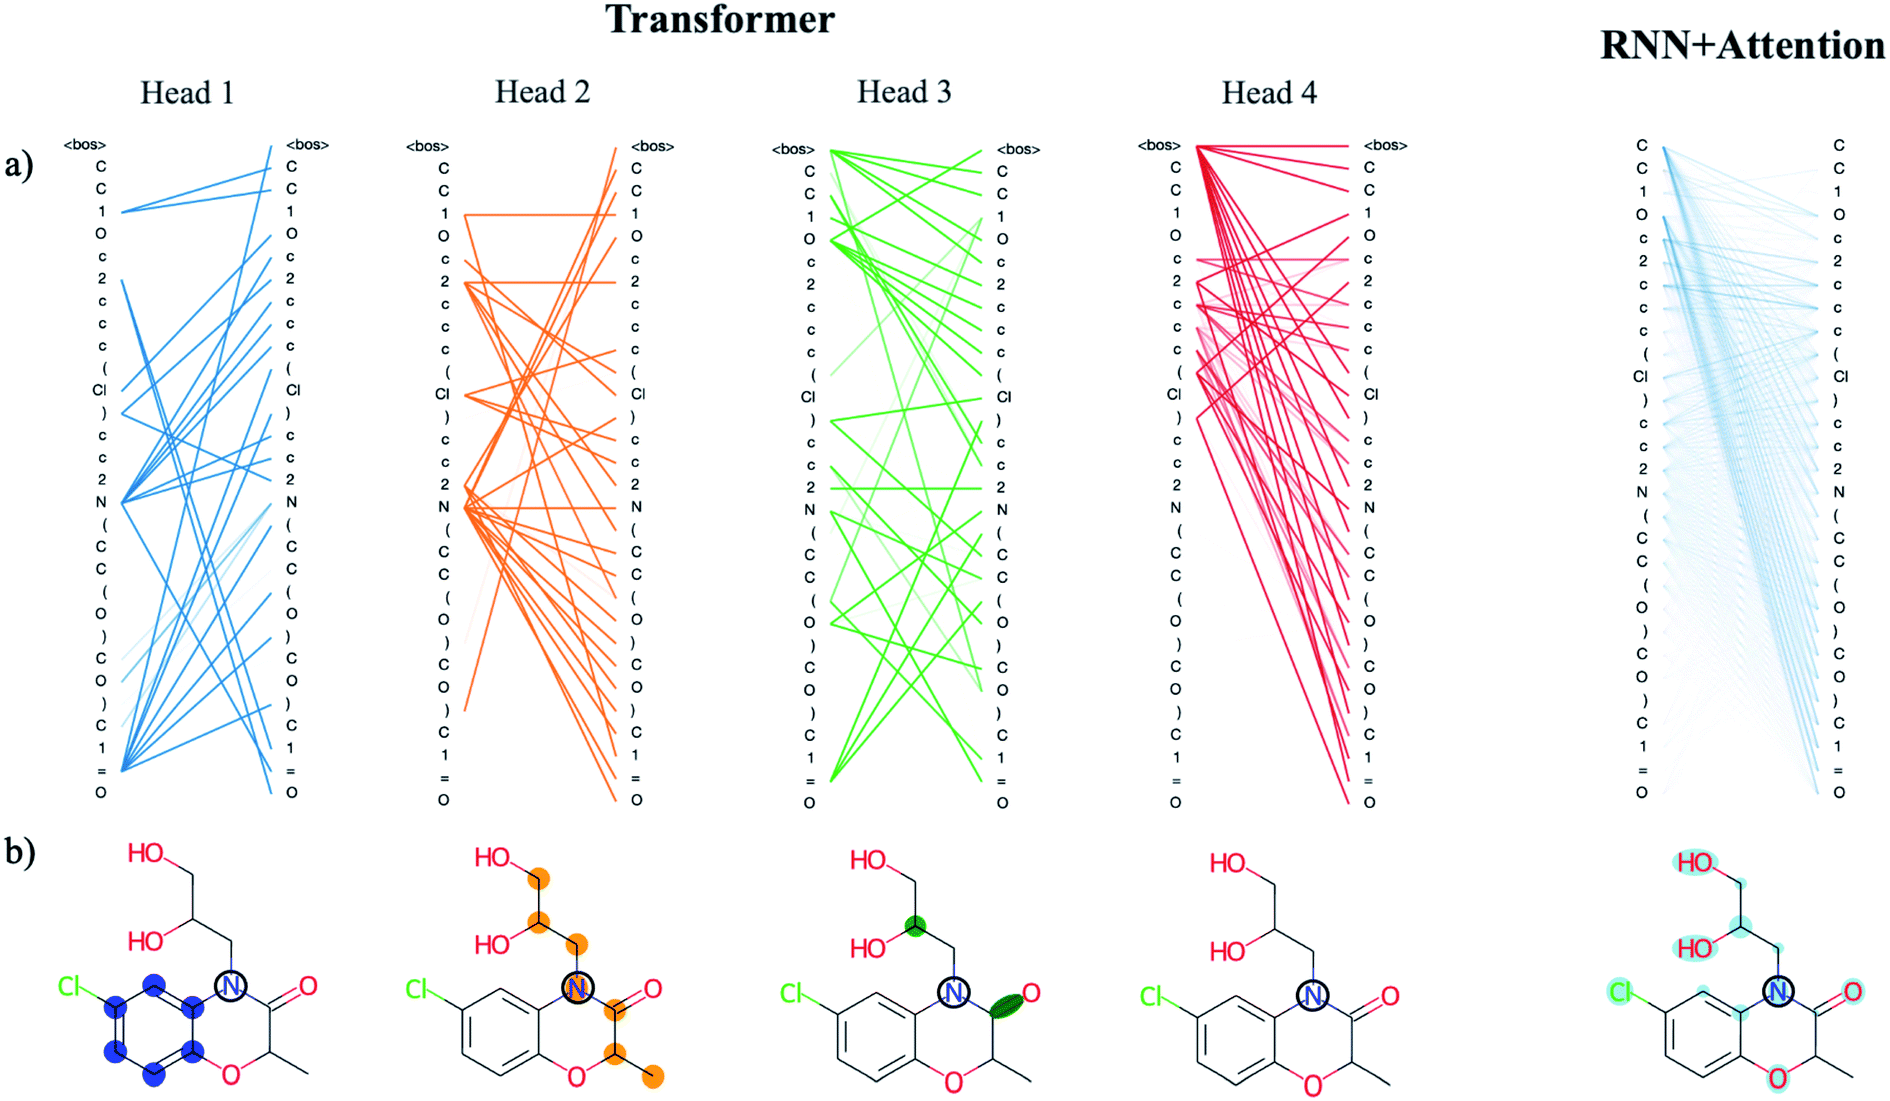
\includegraphics[trim=0 0 18cm 0, width=\textwidth]{./png/interpretability.png}
      \caption{Transformer Orion Dollar et. al. \label{fig:TRANSFORMER}}
    \end{subfigure}
\end{figure}

\end{frame}



\begin{frame}{Object Detection}
\begin{figure}
\centering
\caption{Project's Development Stages}
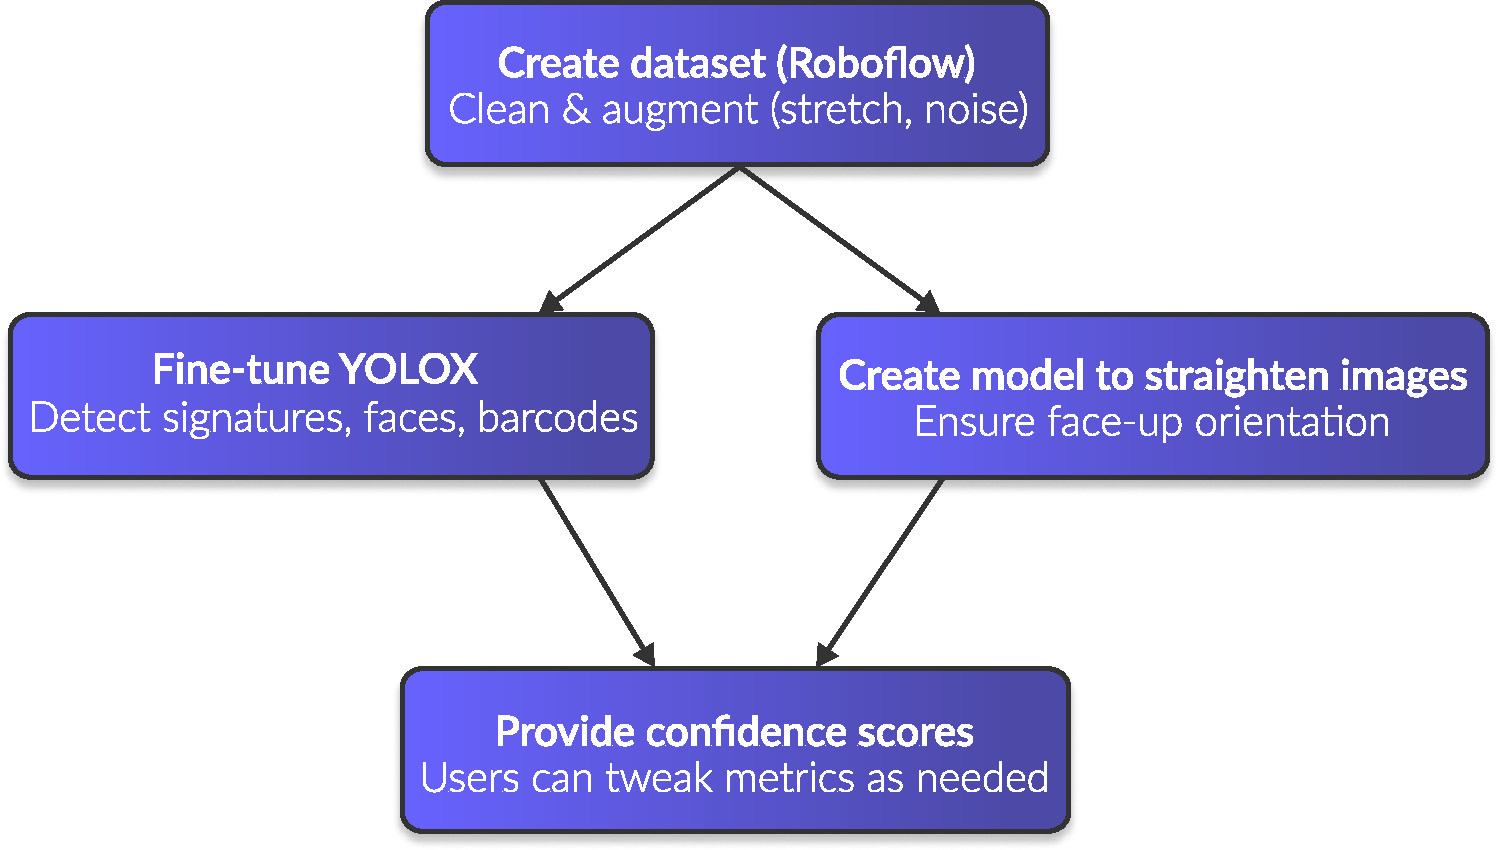
\includegraphics[width=0.8\textwidth]{./flow.pdf}
\end{figure}
\vspace{0.8em}
\hrule
\vspace{0.4em}
\footnotesize{YOLOX: \url{https://github.com/Megvii-BaseDetection/YOLOX}}
\end{frame}


\begin{frame}{Object Detection}
  \begin{itemize}
    \item[] Pseudonymisation of Identity Documents at Zakodium.\footnote{Demo: \url{https://mrz.zakodium.com/}}
    \item[] Frameworks: Tensorflow.js \tf{}, Pytorch \pytorch{}.
  \end{itemize}
\pause
\vspace{0.6em}
\begin{figure}
\centering
\begin{subfigure}[t]{0.4\textwidth}
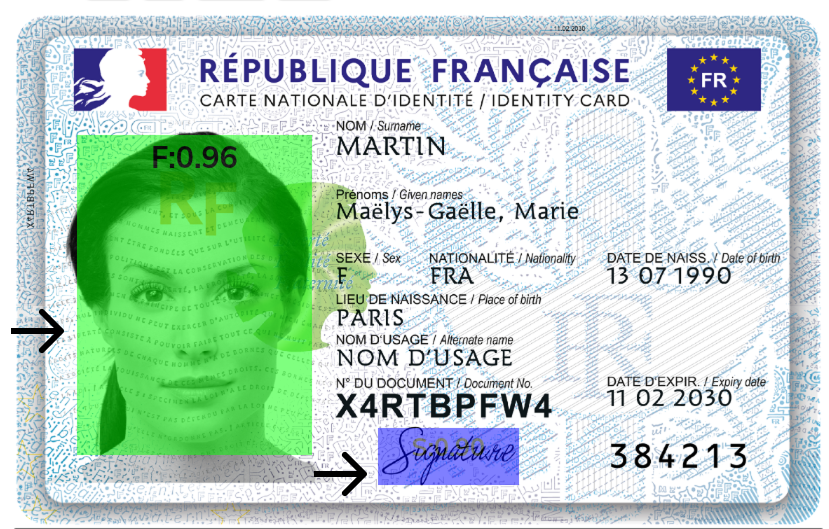
\includegraphics[width=\textwidth]{./png/face_signature_detection_highlighted.png}
\caption{Face and signature detection\label{fig:face}}
\end{subfigure}
\pause
\begin{subfigure}[t]{0.4\textwidth}
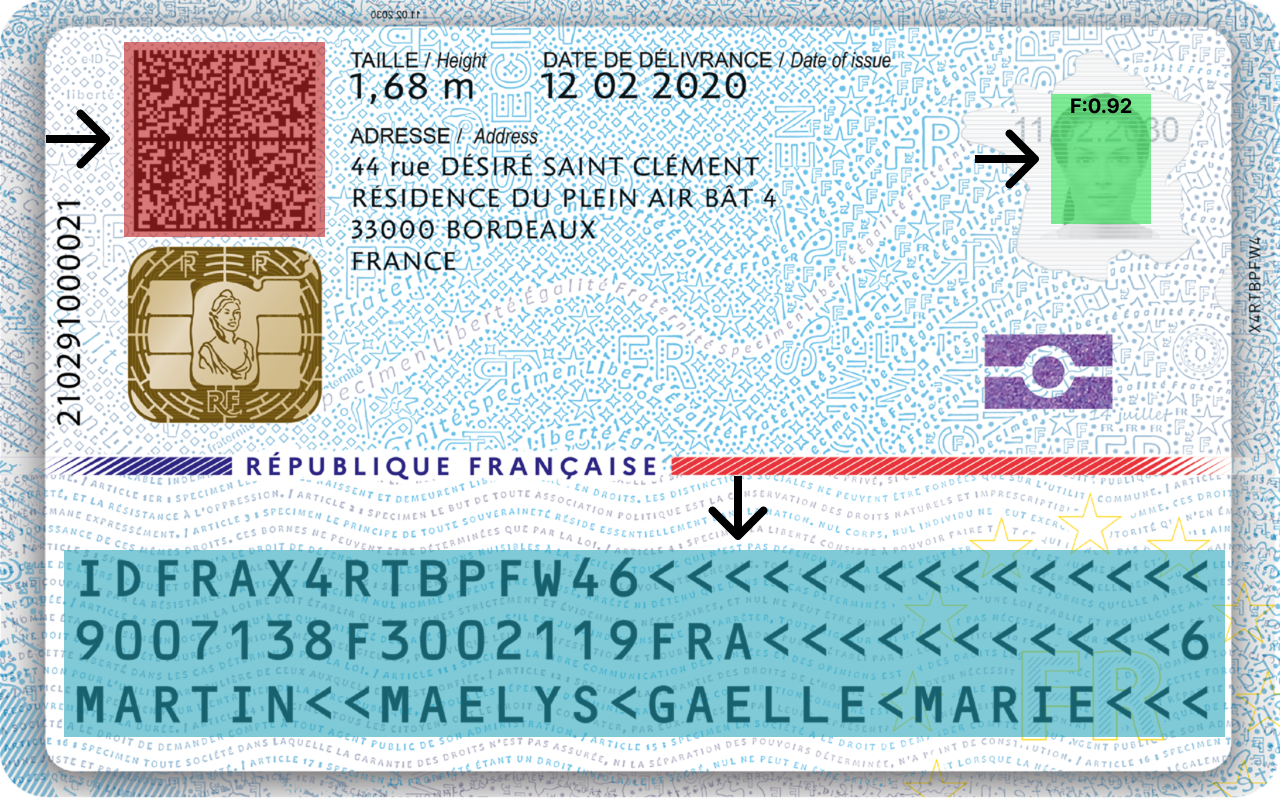
\includegraphics[width=\textwidth]{./png/face_barcode_mrz_detection_highlighted.png}
\caption{Face, barcode, MRZ detection\label{fig:barcode}}
\end{subfigure}
\pause
\caption{\copyright{} European Union, 1998--2026.}
\end{figure}
\end{frame}

\begin{frame}[fragile]{Binary Data Manipulation - iobuffer}
\texttt{iobuffer} is a helper to write binary parsers.

\begin{minted}[bgcolor=Beige,highlightlines={4,9}]{typescript}

import { IOBuffer } from 'iobuffer';

const io = new IOBuffer() // offset 0
io.writeChars('Hello world') // offset now 11
  .back(2) // Back to 9
  .skip(1) // Forward to 10
  .rewind() // back to 0
  .readArray(11, "uint8") // read 11 bytes at once

\end{minted}

\textit{Contributions}: text decoder, readArrays of typed-data, host-endianness detection.

\end{frame}



\begin{frame}{Other Projects}
\small
Base URL for projects: \url{https://github.com/santi-mir/<project>}. \vspace{1.5em}

\begin{tabular}{lcp{3.5cm}}
  \github{} Github Project & \npm{} npm $\downarrow$ & Description \\[0.3em]
  \hline
  \noalign{\vskip 0.5em}
  \texttt{iobuffer} & \iobuffer{}  & Binary data manipulation library \\[0.6em]
  \texttt{regression-simple-linear} & \regression{}  & Simple linear regression \\[0.6em]
  \texttt{regression-polynomial} & \regressionp{}  & Polynomial regression \\[0.6em]
  \texttt{fcnnls} & \fcnnls{}  & Fast combinatorial non-negative least squares \\[0.6em]
  \texttt{spc-parser} & \spc{}  & GRAMS \texttt{.spc} parser \\[0.6em]
  \texttt{wdf-parser} & \wdf{}  & WDF Raman file parser \\[0.6em]

\hline
\end{tabular}

\vspace{1.5em}
Most are also published in Zenodo.

\end{frame}

\begin{frame}{External Image Sources}
\begin{itemize}
  \setlength\itemsep{2em}
  \item ID cards, Figs. \ref{fig:face} and \ref{fig:barcode}: \url{https://commons.wikimedia.org/wiki/Category:Identity_cards_of_France}
  \item VAE (2018) Fig. \ref{fig:VAE}: \url{https://pubs.acs.org/doi/full/10.1021/acscentsci.7b00572}
  \item Transformer (2021) Fig. \ref{fig:TRANSFORMER}: \url{https://pubs.rsc.org/en/content/articlehtml/2021/sc/d1sc01050f}, the image was modified (cropped) to fit into the slide.
\end{itemize}
\end{frame}
\begin{frame}
\begin{center}
Thanks!
\end{center}
\end{frame}
\end{document}
